\documentclass[twocolumn,traditabstract]{aa}\\
\textbf{}\usepackage{fixltx2e}
\usepackage[english]{babel}
\usepackage{graphicx,amsmath}
%\usepackage{epstopdf}
\usepackage{epsf,color}
\usepackage[mathscr]{eucal}
\usepackage{amsmath}
\usepackage{amssymb,amsfonts}
\usepackage{natbib}
\usepackage{txfonts}
\usepackage{dsfont}
\definecolor{Mygreen}{rgb}{0.00, 0.72, 0.0}
\definecolor{Mypink}{rgb}{1.0, 0.0, 0.5}
\usepackage[breaklinks, citecolor=blue, linkcolor=Mygreen, urlcolor=Mypink, colorlinks=true, debug, baseurl=' ']{hyperref}
\usepackage{float}
\usepackage{color}
%\usepackage{scrextend}
%\usepackage{nccmath}
%\usepackage{mathtools, cuted}
%\usepackage{lscape}
\usepackage{widetext}
%\usepackage{flushend}
%\usepackage[T1]{fontenc}\\
\bibpunct{(}{)}{;}{a}{}{,}

\usepackage[style=numeric,maxcitenames=2,
backend=biber,natbib=true]{biblatex}


\begin{document}
\title{Improved mm-wavelength interferometry for Kinetic Inductance Detectors}

\author{A. Fasano \inst{\ref{Neel}},\thanks{Corresponding author: Alessandro Fasano, \url{alessandro.fasano@neel.cnrs.fr}}
	\and M. Aguiar \inst{\ref{IAC}} 
	\and A. Benoit \inst{\ref{Neel}} 
	\and A. Bideaud \inst{\ref{Neel}} 
	\and O. Bourrion \inst{\ref{LPSC}}
	\and M. Calvo \inst{\ref{Neel}}
	\and A. Catalano\inst{\ref{LPSC}}
	\and A. P. de Taoro \inst{\ref{IAC}} 
	\and G. Garde \inst{\ref{Neel}} 
	\and A. Gomez$^4$ 
	\and M. F. Gomez Renasco \inst{\ref{IAC}} 
	\and J. Goupy \inst{\ref{Neel}} 
	\and C. Hoarau\inst{\ref{LPSC}}
	\and R. Hoyland \inst{\ref{IAC}}  
	\and J. F. Mac\'ias-P\'erez\inst{\ref{LPSC}} 
	\and J. Marpaud\inst{\ref{LPSC}} 
	\and A. Monfardini \inst{\ref{Neel}}
	\and G. Pisano \inst{\ref{Cardiff}}  
	\and N. Ponthieu\inst{\ref{IPAG}} 
	\and J. A. Rubi\~no Mart\'in$^3$ 
	\and D. Tourres\inst{\ref{LPSC}} 
	\and C. Tucker \inst{\ref{Cardiff}} 
	\and A. Beelen\inst{\ref{LAM}} 
	\and G. Bres \inst{\ref{Neel}} 
	\and M. De Petris\inst{\ref{Roma}}
	\and P. de Bernardis\inst{\ref{Roma}} 
	\and G. Lagache\inst{\ref{LAM}} 
	\and M. Marton\inst{\ref{LPSC}} 
	\and R. Rebolo \inst{\ref{IAC}} 
	\and S. Roudier\inst{\ref{LPSC}}
}

\institute{
	Institut N\'eel, CNRS and Universit\'e Grenoble Alpes, France
	\label{Neel}
	\and
	Laboratoire de Physique Subatomique et de Cosmologie, Universit\'e Grenoble Alpes, CNRS/IN2P3, 53, avenue des Martyrs, Grenoble, France
	\label{LPSC}
	\and
	Instituto de Astrofísica de Canarias, C/Vía Láctea s/n, E-38205 LaLaguna, Tenerife, Spain
	\label{IAC}
	\and
	Dipartimento di Fisica, Sapienza Universit\`a di Roma, Piazzale Aldo Moro 5, I-00185 Roma, Italy
	\label{Roma}
	\and
	Univ. Grenoble Alpes, CNRS, IPAG, F-38000 Grenoble, France 
	\label{IPAG}
	\and
	Astronomy Instrumentation Group, University of Cardiff, UK
	\label{Cardiff}
	\and
	Aix Marseille Universit\'e, CNRS, LAM (Laboratoire d'Astrophysique de Marseille) UMR 7326, 13388, Marseille, France
	\label{LAM}
}	

	
\abstract{

\emph{Context.} 
Major features demanded for instruments in contemporary cosmology are high mapping speed to cover large portion of the sky and multi-frequency capability for the components separation. In order to simultaneously satisfy the two conditions it is possible to design large arrays of photo noise limited detectors that garatee a high fill-factor and sensitivity. In addition it is desiderable to adopt an interferometer that that allows wide instantaneous Field of View (FoV). In this framework we developed KISS (KIDs Interferometer Spectrum Survey), a spectrometric-imager dedicated to the secondary anisotropies of the Cosmic Microwave Background (CMB).

\emph{Method.} We exploit a Fourier Transform Spectrometer (FTS) with a double-array sensitive to all the interested band: each pixel receives the whole EM signal and the interferometric technique reconstructs the spectrum the instrument is installed in QUIJOTE telescope in Tenerife. The single interferometric figure must be acquired with a stable background to properly convert it in a spectrum where the noise does not become indistinguishable from the signal. Especially for ground-based experiments, the atmosphere background fluctuations require to use low time-constant detectors and fast FTS technology. KISS adopts, for this purpose, two arrays of Kinetic Inductance Detector (KID) coupled to a Martin Puplett Interferometer (MPI).

\emph{Aims.} In this paper we describe the solution adopted to improve the conversion accuracy of the instrument from I,Q to Hz signal to overcome to non-linear response.

\emph{Results.} We first demonstrate the feasibility of this technique with a simulation. We, then, study the performance of such technique, applying it to on-sky observations. The acquisition technique has been qualified during the commissioning campaign during 2019/2020 in Tenerife. It represents a solution for fast interferometers acquisition experiments exploiting KID based interferometer.

}

\keyword{instrumentation: detectors - methods: observational simulation - telescopes - techniques: photometry, interferometry}
	
\maketitle

\section{Introduction}

Foregrounds subtraction and components separation in mm-wavelength astronomy require simultaneous observation. This scenario suggests the choice of FTS: this technique exploits the interference of light rather than separate the wavelengths and, compared to competitors (on-chip (\cite{deshima}) and grating (\cite{grating}) spectroscopy) allows larger instantaneous FoV.

KISS is a fast spectrometer based on KID (for an overview see \cite{kids}) and installed at the 2.25 m QUIJOTE telescope (see \cite{fasano-ltd} and \cite{fasano-nika2} for the instrument description). Firstly, as in the past for FIRAS (\cite{FIRAS}), the selection of the FTS for the will of developing an instrument fells on a MPI: an interferometer that measures the difference between the powers of two input beams (\cite{mpi}). The MPI transposes the observing frequencies paradigm from time to spacial domain and allows to use a conversion source: an ideal choice for precise measurements.
Secondly, the necessity to go fast on data acquisition makes suitable to choose fast detectors like KID. Taking in consideration these premises, using a ``brute-force'' acquisition technique, where you stock all the information available, would result on a huge data production. Starting from this scenario, it is desirable to adopt a smart solution that minimises the amount of data.
In the case of dual band photometers, such as ground-based NIKA \cite{Monfardini_2010:NIKA} and NIKA2 \cite{nika2}, the acquisition rate at 23.48 Hz allows to average the points and obtain a conversion, for KISS the premises are different: it is a spectrometer. It cannot average because of the rapid background fluctuations and the interferometric signal that is an equivalent multi-channel photometer at 4 Hz.

In sec.~\ref{sec:kid} we describe the KID and we show the properties of KISS arrays. 
In sec.~\ref{sec:photo} we introduce the method used in past for NIKA2 for conversion and tuning. In the same section, it is described the new method for KISS, the data implementation and the algorithm.
In the sec.~\ref{sec:results}  we show two results: the observational simulation and the application of the method on real data. In the sec.~\ref{subsec:moon} we apply the conversion to on-sky data.

\section{KID properties}
\label{sec:kid}

The KID a is high quality factor superconducting resonator exploited as detector in mm-wavelength. It is based on the change of kinetic inductance with an incoming radiation, that is inversely proportional to the density of Cooper pairs. It is read-out by a bias line injecting a tone at its correspondence resonant frequency; at this peculiar frequency, in fact, the coupling between the resonator and the readout line results in an energy absorption, aka band-stop filtering that can be monitored. Its time constant is fixed by the recombination time of the quasi-particles (few $10$ $\mu s$). This represents a major advantage with respect to competitors that are, indeed, a factor $\gtrsim$10 slower.

The $S_{21}$ signal (output/input ratio) related to the KID detector is studied in the complex plane In-phase and Quadrature $(I,Q)$, where the resonance shape corresponds to a circle.
The conversion of the $(I,Q)$ signal to absorbed optical power is one of the most difficult challenge using KID and it represents a different issue to readout, e.g., thermal detectors (bolometer, TES et cetera).

We use the following  values to characterise the resonator: the resonance frequency ($f_0$), the internal quality factor ($Q_i$) and the coupling quality factor ($Q_c$). In order to fit the resonance we use the skewed Lorentzian profile \cite{Gao}:

\begin{equation}
\left|S_{21}(f)\right|= A+B(f-f_0)+\frac{C+D(f-f_0)}{1+4Q_{tot}^2\cfrac{(f-f_0)^2}{f_0^2}} \text{ ,}
\label{eq:s21_amp}
\end{equation}

\noindent where $A$, $B$, $C$ and $D$ are factors that do not influence the parameters under study. We can, thus, characterise the pixels. With eq. \ref{eq:s21_amp} we can extrapolate $Qi$ (\cite{Gao}):

\begin{equation}
Q_i =\frac{Q_{tot}}{min(\left|S_{21}(f)\right|)}	\text{ .}
\end{equation} 

In fig. \ref{fig:fit_amp} and \ref{fig:hist} we show the electrical measurements for the KISS arrays performed in laboratory.

\begin{figure}[htf]
	\centering
	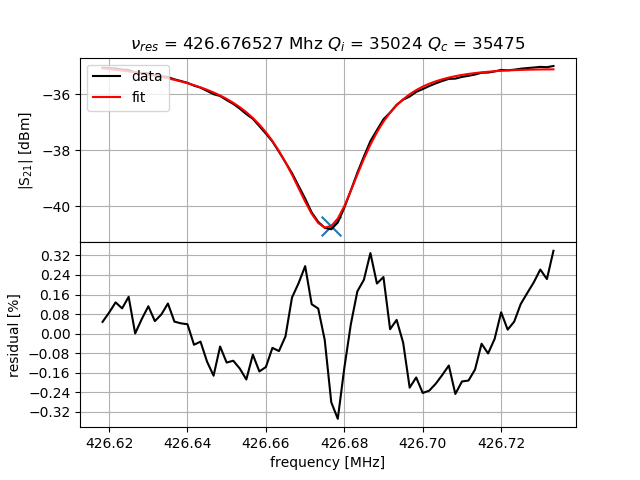
\includegraphics[width=.5\textwidth]{3.acqui/resonance_fit.png}
	\caption{Up: single pixel bias signal data (in black) fitted (in red) by eq. \ref{eq:s21_amp}. Bottom: percentile residual between fit and data.}
	\label{fig:fit_amp}
\end{figure}

\begin{figure}[htf]
	\centering
	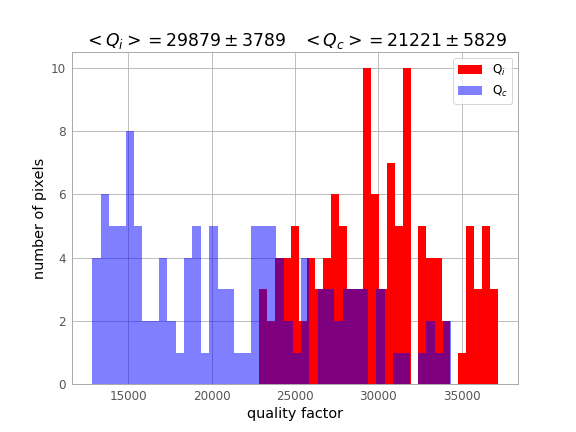
\includegraphics[width=.5\textwidth]{3.acqui/Q_hist.png}
	\caption{Quality factors histograms measured on the KISS array. In red the internal quality factor ($Q_i$) with a background of 50 K that simulates the sky and in blue the coupling quality factor ($Q_c$).}
	\label{fig:hist}
\end{figure}

\noindent In terms of the previous parameters, the pixel design answers to the necessity of particular specifications: the resonance frequency ($f_0$) is in agreement with the amplifier working range and the coupling quality factor ($Q_c$) is coupled to the internal one ($Q_i$), that is related to background, to maximise the responsivity (as demonstrated in \cite{Gao}).

\section{Photometric response}
\label{sec:photo}

\subsection{2-point modulation technique}
\label{2-point}
Smart readout technique is required to properly study the signal following fluctuating background. In the past, e.g. for NIKA, an innovative readout technique has been developed (see \cite{Calvo2013} for a detailed discussion): the 2-point modulation technique.
The idea, as described in \cite{Catalano2014} , has been to replace the standard fixed excitation (single frequency) tone with a modulated input based on two different frequencies separated by $f_{LO}$: 

\begin{equation}
\begin{align}
f_+ = f_0 + \delta f_{LO}/2 \text{ ,}
\\
f_- = f_0 - \delta f_{LO}/2 \text{ ,}
\end{align}
\end{equation}

\noindent where $f_0$ is the resonant frequency. This modulation is synchronised to the FPGA sampling of the signal at $\sim$24 Hz. Each raw data point is composed by $(I(t), Q(t))$ values and the corresponding differential values:

\begin{equation}
\left( \frac{dI}{df}(t),\frac{dQ}{df}(t) \right) = \left( \frac{I(f_+)-I(f_-)}{\delta f_{LO}}, \frac{Q(f_+)-Q(f_-)}{\delta f_{LO}} \right) \text{ .}
\label{eq:didq}
\end{equation}

\noindent In this way, if a variation $(\Delta I(t), \Delta Q(t))$ occurs between two successive points, it is possible to estimate the corresponding shift in the resonant frequency ($\Delta f_0(t)$) by projecting
$(\Delta I(t), \Delta Q(t))$ along the gradient found, using 
eq. \ref{eq:didq}:

\begin{equation}
\Delta \hat{f}_0 (t) = \frac{(\Delta I(t), \Delta Q(t))\cdot (dI/df(t),dQ/df(t)  ) }{ ( dI/df(t), dQ/df(t) )^2 }\cdot\delta f_{LO} \text{ ,}
\end{equation}

\noindent we refer to $\Delta \hat{f}_0 (t)$ as $RFdIdQ$.

\subsubsection{Tuning procedure}
\label{sec:tuning}

The 2-point modulation technique, described in subsec.~\ref{2-point} is the major improvement on the data conversion. On the other side, to optimise the working point of the KID it is necessary to retune: while you observe, the atmospheric fluctuations modify the resonance. What is done at the end of each observation, in the standard perspective, is a full frequency sweep to retune the resonance frequency: this represents a time-demanding procedure. It is possible to adopt a strategy that permits to save $\sim$75\% of time in the pre-observation phase of retuning, this strategy is detailed explained in (\cite{2014SPIE.9153E..02C}). At first, you measure the angle $\Phi$ between the vectors $(I,Q)$ and $(dI/df_{LO},dQ/df_{LO})$ referring to eq. \ref{eq:didq} and you define, for convenience, a new angle $\theta\doteq \pi/2-\Phi$ that changes smoothly around $[-\pi,\pi]$. Secondly, the excitation tone is fixed at $\theta=0$ and you estimate the $\theta(f)$ slope $\Delta\theta/\Delta f'$. Then, you vary the tone frequency $f^i$ monitoring $\theta^i$. And finally, you can evaluate the new resonance frequency:

\begin{equation}
f^i_0 \simeq f^i - \frac{\theta^i(t)}{\Delta\theta/\Delta f'} \text{ .}
\end{equation}

The procedure described in this section is a resilient tool that can be adopt on photometric KIDs-based experiments: even for large background fluctuations, you can iterate the algorithm to converge.

\subsection{3-point modulation technique}

The constraints over the data acquisition are slightly more demanding in KISS: two consecutive interferograms are acquired at 5 Hz, to overcome the 1/f atmospheric noise at $\sim$1 Hz, and the data rate is quite higher (3.816 kHz) in order to obtain the aimed spectral resolution of few GHz. In this condition it is not possible to modulate each single point signal, because the FPGA does not reach the necessary rate and you would, eventually, manage a factor 2 on data weight.\\
As previously mentioned, we cannot use the same technique, described in the subsec.~\ref{2-point}, for interferometry. The acquisition rate is not high enough to average successive interferogram points and the continuous presence of interferometric signal would introduce, with such a technique, a systematic on the spectrum calculus. We record the (I,Q) signal related to the phase signal\footnote{$\phi = \arctan \left( \frac{I}{Q} \right) $ .}. Notwithstanding, the background fluctuations (with respect to stable conditions of stratospheric balloons and satellites) for on-ground experiments makes the phase not suitable for its non-linearity. The resonance frequency data [Hz] preserve the linear regime, it is thus necessary to convert the phase to frequency. We modulate the signal at the beginning of each interferogram to obtain two frequency calibration points known a priori.

\subsubsection{Implementation}
The spectral information is organised in data block containing forward and backward interferogram: a moving mirror oscillates generating the optical path difference that results in the interferogram figures, one per oscillation direction (see \cite{fasano-ltd} for the detailed discussion). The data blocks are continuously acquired on-the-fly during the astronomical observations, they are singularly related to a specific point on the sky. This repetitive points sequence is preceded by a first part where there are injected two calibrating frequencies (as introduced before), respectively:
\begin{equation}
\begin{align}
f_+ &= f_0 + \Delta f_{LO}/2 	\text{ ,}
\\
f_- &= f_0 - \Delta f_{LO}/2	\text{ ,}
\end{align}
\label{eq:fmod}
\end{equation}

\noindent during this modulation the sweeping mirror is fixed (it does not introduce an optical path). The rest of the points are fixed at the tuned resonance frequency $f_0$ \footnote{In the beginning of each map-making the resonance frequency is optimised for the current background.}, as we can see in fig. \ref{fig:mod}.

\begin{figure}[htf]
	\centering
	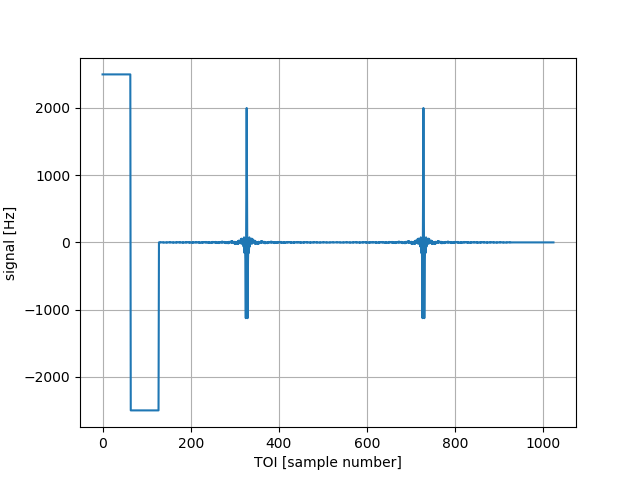
\includegraphics[width=.5\textwidth]{3.acqui/block_data.png}
	\caption{Data block simulation of KISS: signal [Hz] vs sample number. There are a total of 1024 points: the first 128 dedicated to the modulation and the rest to incoming signal. We simulate the forward and backward interferograms with a typical amplitude of 2 kHz and input black body sources at 3 K and 30 K respectively.}
	\label{fig:mod}
\end{figure}

\noindent The choice over the total number of points for one single block, including the ones assigned to the modulation, takes into account few major constraints.

\noindent \color{red} There are two scientific and one instrumental requirements:

\begin{itemize}
	\item 1.5 GHz EM resolution;
	\item (80)110-300 GHz EM band\footnote{The lower limit at 80 GHz is for the Ti-Al bilayer absorber.};
	\item 4 Hz sweep of the moving mirror to overcome the atmospheric pink noise\footnote{The pink (1/f) atmospheric signal presents a low-frequency noise spectrum with a typical knee at $\sim$1 Hz.}.
\end{itemize}
\noindent
For the first requirement we need at least 5 cm of MPI moving mirror displacement, Optical Path Difference (OPD).
For the second one we  400 $\mu$m of step precision of step precision
#points = 5 cm / 400 μm of step precision x2 = 250 points
x2 factor for the forward and a backward interferogram

250 points x 4 Hz = 1 kHz

We are at 4 kHz: we took margin exploiting FPGA max
The drawback is to have a precision on the injected tone of 4 kHz

Maximum performances available: 8.5 cm -> 0.8 GHz

The maximum frequency depends on the single point sampling:

\begin{equation}
	\Delta x = \frac{1}{2\sigma_{max} }
\end{equation}

\color{black}

the spectral resolution aimed to $\sim$1 GHz requires a displacement of the mirror of 10 cm; the cut-off of the KID time constant (few 10 $\mu$s), that limits the single datum acquisition rate; the fast (5 Hz) scan requirement to avoid the 1/f atmospheric noise. The result consists on a total period of 1024 points, where each point is acquired at 3.816 kHz, dedicating the first 128 to the modulation. In this way we have $\sim$400 points each interferogram, obtaining $\sim$100 points on the interested spectrum band (80-300 GHz).\\



\subsubsection{Conversion algorithm}
\label{conv}

\noindent We can extrapolate the conversion factor $C$ [Hz/rad] through a circular fit on the modulation points $(x_1,y_1)$ and $(x_2,y_2)$, and the baseline point $(x_3,y_3)$, referring to fig. \ref{fig:IQ_modulation}.

\begin{figure}[htf]
	\centering
	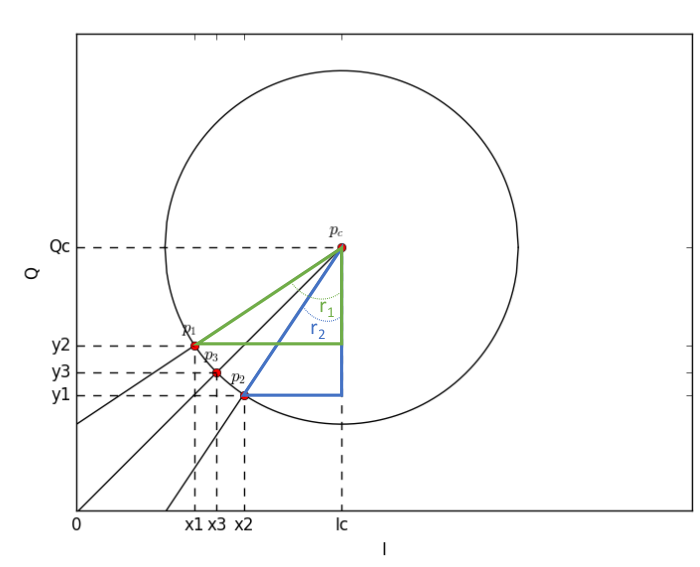
\includegraphics[width=0.4\textwidth]{3.acqui/circle.png}
	\caption{Resonance circle in the $(I,Q)$ plane. $p_1$ and $p_2$ are the modulation points, $p_3$ is the measurement point and $p_c$ is the circle centre. }
	\label{fig:IQ_modulation}
\end{figure}


We obtain, in this way, the coordinates of the circle centre $(I_c,Q_c)$. We can calculate, thus, the $r_1$ and $r_2$ angles as following:

\begin{equation}
\begin{align}
r_1 &= \arctan\left( \frac{I_c-x_1}{Q_c - y_1}  \right) &\text{ ,}\\
r_2 &= \arctan\left( \frac{I_c-x_2}{Q_c - y_2}  \right) &\text{ .}
\end{align}
\end{equation}

\noindent The conversion factor $C$ is, then, obtained by:

\begin{equation}
\begin{align}
\Delta \phi &= r_2-r_1 &\text{ ,}\\
C&=\Delta f_c/\Delta\phi &\text{ ;}
\end{align}
\end{equation}

\noindent where $\Delta f_c$ is the modulation factor in hertz set by the injecting tone, known a priori, ($\Delta f_c = 2\Delta f_{LO}$ from eq.~\ref{eq:fmod}).

Operatively, $C$ converts the observing phase $\phi$ to $f'$ hertz data. We first calculate the $r$ angle:


\begin{equation}
r = \arctan \left( \frac{I_c - I}{Q_c - Q} \right) \text{ .}
\end{equation}

\noindent In the end, we obtain the frequency data:

\begin{equation}
f' = C \cdot r \text{ .}
\end{equation}

\noindent This represents, indeed, the physical quantity that can be directly converted to incoming power (as seen in \cite{Swenson}).


\section{Results}
\label{sec:results}

\subsection{Validation with simulation}

The first step to validate the conversion technique has been the simulation of the KID pixel used for KISS, qualifying it for the modulation technique.
The $S_{21}$ signal of the KID resonator, in the complex plane is described by the equation (\cite{Gao}):

\begin{equation}
S_{21}(f)=ae^{-2\pi j f \tau} \left[ 1-\frac{\frac{Q_{tot}}{Q_c}e^{j\phi_0}}{1+2jQ_{tot}\left(\frac{f-f_0}{f_0}\right)}\right] \text{ ,}
\label{eq:s21_IQ}
\end{equation}

\noindent where , $Q_{tot}\doteq\left( 1/Q_i + 1/Q_c \right)^{-1}$ and $\mathfrak{R}$ is the responsivity measured; $\tau$ is the retard introduced by the cables and $\phi_0$ is a phase, and these last two parameters are not taken into account for this study.

\begin{table}[htf]
	\footnotesize
	\centering
	\caption{Input values from laboratory characterisation taken from the analysis showed in fig. \ref{fig:hist} and discussed in subsec.~\ref{sec:kid}.}
	\begin{tabular}{cc}
		\toprule
		\textbf{parameter} & \textbf{value} \\
		\toprule
		$\tau$ & 1 \\ 
		\midrule 
		$\phi_0$ & 0 \\
		\midrule
		$f_0$ & 500 MHz \\  
		\midrule 
		$Q_i$ & 30'000 @ 50 K \\ 
		\midrule 
		$Q_c$ & 21'000 \\ 
		\midrule 
		$\mathfrak{R}$  & 1.5 kHz/K \\ 
		\bottomrule
	\end{tabular}
	\label{tab:s21_values}
\end{table}

\noindent We can use, then, the eq.~\ref{eq:s21_IQ} inserting the laboratory values in tab.~\ref{tab:s21_values} to obtain the $S_{21}(f)$ simulated signal, whose module is shown in fig. \ref{fig:s21_simu}.

\begin{figure}[htf]
	\centering
	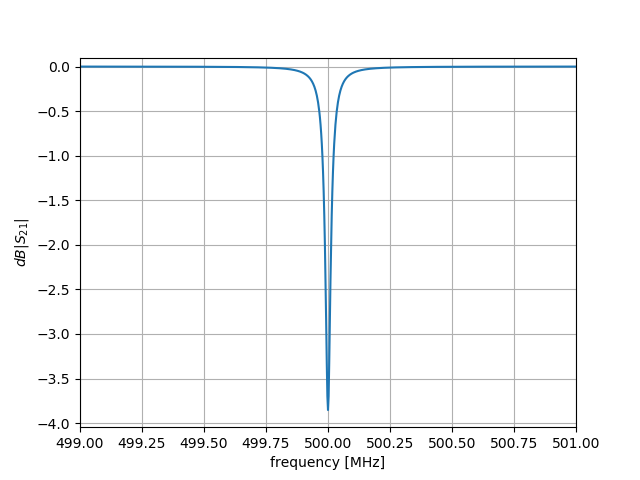
\includegraphics[width=.5\textwidth]{3.acqui/resonance.png}
	\caption{$\left|S_{21} \right|$ signal [dB] (simulated using eq.~\ref{eq:s21_IQ} with input values of tab.~\ref{tab:s21_values}) vs frequency [MHz]. It represents the typical KISS pixel.}
	\label{fig:s21_simu}
\end{figure}

First of all, starting from these simulated data we generate a data block with assigned modulation factor and interferogram amplitude ($A$) in hertz. The second step is to use these hertz data with, again, eq. \ref{eq:s21_IQ} obtaining the values in quadrature $(I,Q)$. From them we compute the phase $\left( \phi=\arctan\left(\frac{I}{Q}\right) \right)$\footnote{ $I = \Re(S_{21})$ and $Q = \Im({S_{21})}$ }. Finally we come back to hertz signal through the conversion algorithm described in subsec.~\ref{conv}. We, thus, compare the modulation factor and interferogram amplitude in input ($C_{in}$ and $A_{in}$) and output ($C_{out}$ and $A_{out}$) of this algorithm. This verification is necessary to understand the reliability of the conversion method. In fig. \ref{fig:cal_bck} we report the change of the conversion factor as a function of background, at fixed modulation factor and interferogram amplitude.

\begin{figure}[htf]
	\centering
	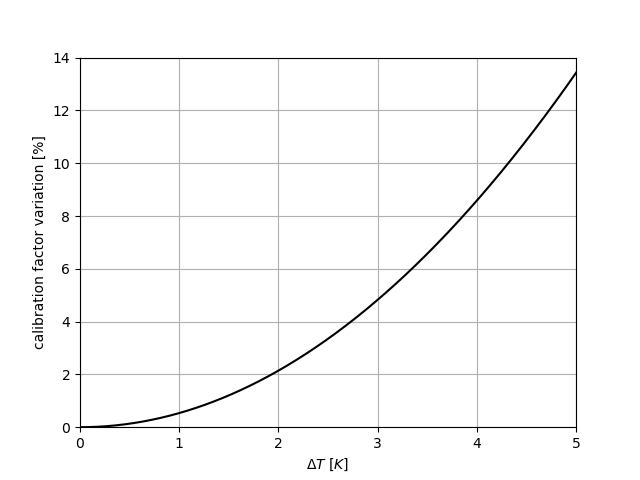
\includegraphics[width=.5\textwidth]{3.acqui/calibration_factor_variation.png}
	\caption{conversion factor percentile variation $\left( \frac{C_{out}-C_{in}}{C_{in}} \right)$ vs background variation [K]. The modulation factor ($\Delta f_c$) is fixed at at 2.5 kHz. The conversion factor ($C_{out}$) is independent from $A_{in}$.}
	\label{fig:cal_bck}
\end{figure}

\noindent In fig. \ref{fig:amp_bck} we show the variation on the estimation of the interferogram amplitude, at fixed modulation factor: we see how this estimation is degradated at large background variations.

\begin{figure}[htf]
	\centering
	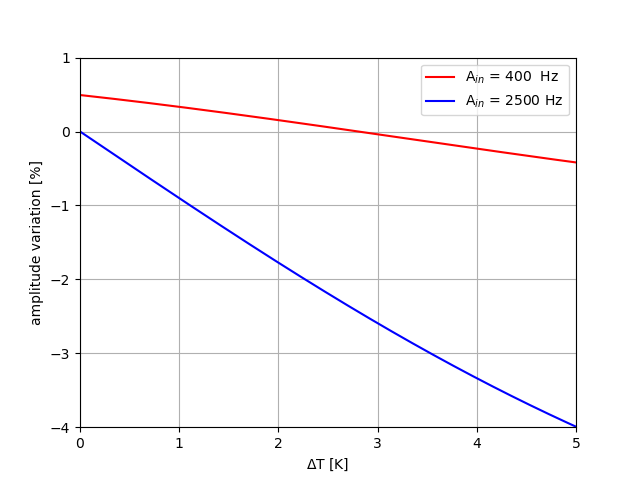
\includegraphics[width=.5\textwidth]{3.acqui/amplitude_variation.png}
	\caption{Interferogram amplitude percentile variation $\left( \frac{A_{out}-A_{in}}{A_{in}} \right)$ estimation vs background [K]. The modulation factor ($\Delta f_c$) is fixed at 2.5 kHz. We can see how the higher value of the amplitude degrades the method.}
	\label{fig:amp_bck}
\end{figure}

\noindent In fig.~\ref{fig:amp_mod} we show the last result of the simulation: every curve is at different, fixed interferogram amplitude and the figure represents the variation on the amplitude estimation in function of different conversion factors. As expected, we want to be as close as possible between the conversion factor and the amplitude variation. Other choices compromise the amplitude estimation of maximum $\sim$1\%.

\begin{figure}[htf]
	\centering
 	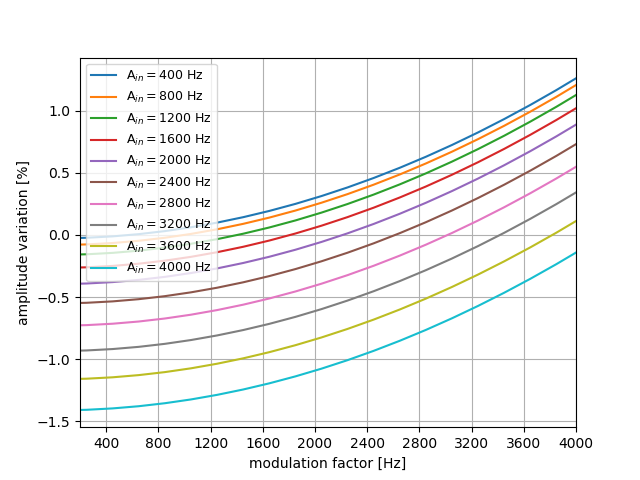
\includegraphics[width=.5\textwidth]{3.acqui/several_modulations.png}
	\caption{Every curve is at different interferogram amplitude ($A_{in}$). Interferogram amplitude percentile variation $\left( \frac{A_{out}-A_{in}}{A_{in}} \right)$ vs modulation factor ($\Delta f_c$).  The background is fixed at zero. We can see how the error on the estimation converges to 0 when $\Delta f_c$ approaches $A_{in}$. }
	\label{fig:amp_mod}
\end{figure}


\subsection{Validation on observational data}
In this subsection we show the results obtained from the commissioning campaign at the telescope. We can see in fig. \ref{fig:circle} the circular fit performed on real data as described in fig.~\ref{fig:IQ_modulation}: the two external are the modulation points and the central distribution represents the variation of the signal during the observation.


\begin{figure}[htf]
	\centering
	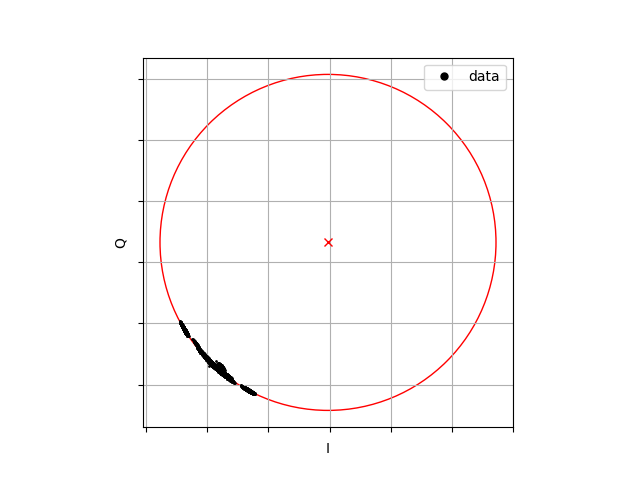
\includegraphics[width=.5\textwidth]{4.results/circular_fit.png}
	\caption{Observation in $(I,Q)$ plan: in black dots the data and in red shape the circular fit. We can see the two modulation (external) points and the central distribution due to the signal changing during the observation}
	\label{fig:circle}
\end{figure}

\noindent Operatively, the circular fit showed in fig. \ref{fig:circle} is used in two different ways and represents a crucial tool during the observations, as well as for the data analysis. Firstly, during the observation, it gives an important visual quick-look feedback to understand if the conversion is correctly working. Secondly, it is one of the first step in the conversion algorithm for the physical data analysis, as already described in subsec.~\ref{conv}.

The first result, that we can compare with the simulation, is reported in fig. \ref{fig:calfact}: it is the conversion factor estimated as a function of sample time during a sky observation. Every point corresponds to a data block (sampled at 5 Hz).

\begin{figure}[htf]
	\centering
	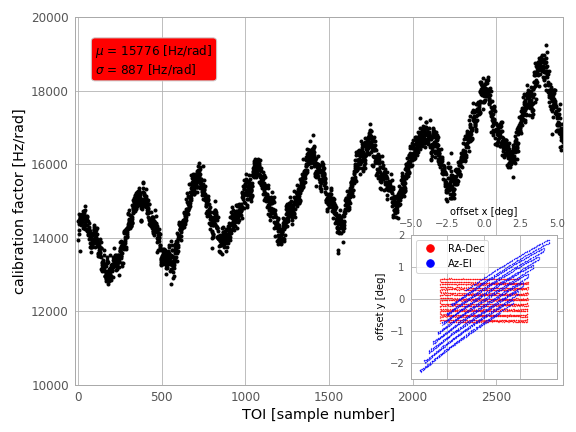
\includegraphics[width=.5\textwidth]{4.results/calfact.png}
	\caption{conversion factor as a function of TOI during an observation. The gaussian fit reported in the red top-left box is evaluated from the data that have been previously median filtered. We can notice the derive of the conversion factor due to the Right Ascension - Declination (RA-Dec) observation: the telescope increases the elevation following the source. In the bottom-right the offset maps of the sky-coordinates in both RA-Dec and Azimuth-Elevation (Az-El).}
	\label{fig:calfact}
\end{figure}


Here we assume the background fluctuation, as seen in fig.~\ref{fig:cal_bck}, as unique source of incertitude for the conversion factor estimation: we consider the noise contamination negligible. Let's first demonstrate this assumption. Following the on-sky results we take the median of the $ASD$ ($\tilde{ASD}$) as its equivalent white noise level: it is, taking margins, $\sim$1 $Hz/\sqrt{Hz}$.
\noindent  We can, then, use the standard deviation definition of the TOI noise signal:

\begin{equation}
\sigma \doteq \int_{0}^{\Delta f} \left[ASD(f) \right]^2\cdot df \text{ .}
\label{eq:sigma}
\end{equation}

\noindent where $ASD(f)$ is the $ASD$ as a function of frequency $f\in[0,\Delta f]$, $\Delta f$ is the bandwidth equal to half of the sampling frequency (for the Nyquist theorem) and $df\doteq\Delta f/N$, where $N$ is the number of the points.

\noindent Approximating $ASD$ in eq. \ref{eq:sigma} as a pure white noise ($\tilde{ASD}$) we obtain:

\begin{equation}
\sigma\simeq \sqrt{ \tilde{ASD}^2 \cdot \Delta f } \text{ ,}
\end{equation}

\noindent Finally, in tab. \ref{tab:sigma_sig}, we can see the typical fluctuations of the signal as a function of sampling rate: compared to the background variation (equivalent of $\sim 1$ kHz) simulation in fig. \ref{fig:calfact} it represents, Q.E.D., a very small components.

\begin{table}[htf]
	\footnotesize
	\centering
	\caption{From eq. \ref{eq:sigma} typical rounded-up 1-$\sigma$ noise signal.}
	\begin{tabular}{ccc}
		\toprule
		\textbf{mode} & \textbf{bandwidth [Hz]} & \textbf{$\sigma$ [Hz]} \\
		\toprule
		single point & 1908 & $\sim$50 \\ 
		\midrule 
		block data & 2 & $\sim$2 \\ 
		\bottomrule
	\end{tabular}
	\label{tab:sigma_sig}
\end{table}

Starting from this paradigm we can compare the results of the simulation with on sky observations. From the simulation we know that there is a $\lesssim 3\%$ variation of the conversion factor each kelvin background fluctuation, as shown in fig. \ref{fig:cal_bck}. What we notice on sky (fig. \ref{fig:calfact}) is a fluctuation $\sigma/\mu\sim6\%$, where $\sigma$ is the standard deviation and $\mu$ the mean value of the conversion factor. We can conclude that during a typical $\sim$4 degree scan we have temperature fluctuation of the sky $\lesssim 2$ K.

Secondly, what we need to state that the acquisition/data-reduction system is qualified for the instrument is to observe the capability of the conversion to adapt to different background (analogously to the autotuning of NIKA/NIKA2 described in subsec.~\ref{sec:tuning}). For this purpose, we take three consecutive maps at increasing elevation: we plot the $(I,Q)$ data of the first subscan for each map observing the behaviour of the acquisition referring the circular fit to the first tuning (corresponding to the first map). The result is shown in fig. \ref{fig:autotuning}.

\begin{figure}[htf]
	\centering
	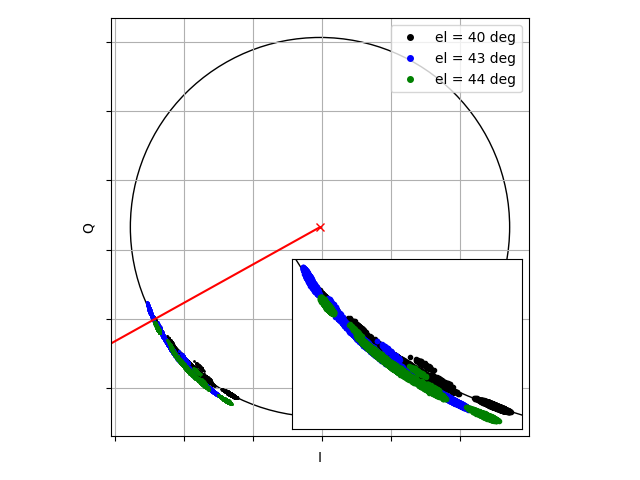
\includegraphics[width=.5\textwidth]{4.results/autotuning.png}
	\caption{$(I,Q)$ signal of the first subscan for three consecutive maps, i.e., increasing elevation. The red straight line is the intercept between the origin and the circle centre.}
	\label{fig:autotuning}
\end{figure}

\noindent We can see how the data are disposed on the same region close to the ones of the first circle, they are around the intercept between the centre of the circle the origin: it means that they are around the minimum of the resonance, i.e., to the frequency of resonance. The data are not perfectly centred because of the intrinsic incertitude on the binning of the injected tone. The radial shift is due to the background change: different elevations correspond to a different air mass ($\sim 1/\cos(el)$). The conversion technique performed between each map recovers the resonance tone, adapting it to the background change.

\subsection{Moon map at different elevations}
\label{subsec:moon}

\begin{equation}
	S_{obs} = S_{corr}\cdot e^{ -\tau \cdot a.m. } 
\end{equation}

\begin{figure}[htf]
	\centering
	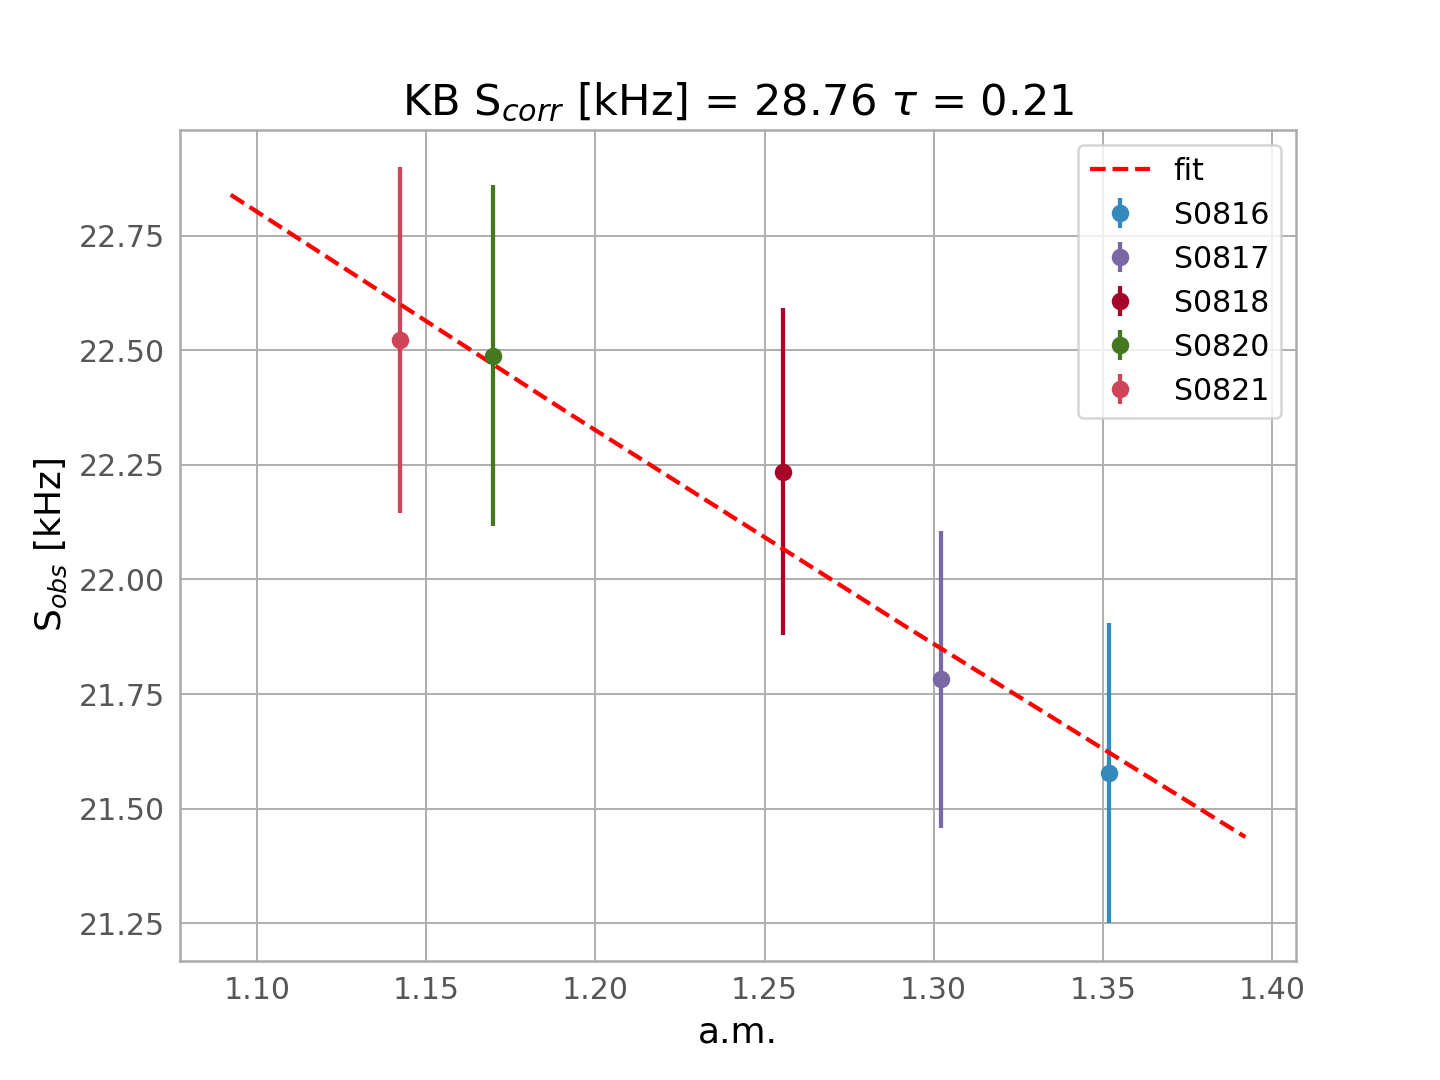
\includegraphics[width=.5\textwidth]{4.results/moon.png}
	\caption{}
	\label{fig:moon}
\end{figure}

\section{Conclusions and Perspectives}
\label{sec:conclu}
The purpose of this paper is to demonstrate and explain the new conversion technique for mm-wavelength interferometric experiment exploiting KID. As previously mentioned, this algorithm is naturally implementable for all those kind of instruments that will aim to exploit KID-based interferometers: a worthwhile solution for the contemporary and future multi-wavelength astronomy. Although KISS represents a standalone instrument to make science, it opens future perspectives for larger arrays experiments, like CONCERTO \cite{concerto}. Specifically for these cases, in fact, our new algorithm will minimise the data production, contain the inflation on the electronics specifications and allow KID exploitation for interferometry.

%\bibliography{bibliography}

\printbibliography

\end{document}

